\documentclass{beamer}
\mode<presentation>
\usetheme{CambridgeUS}
\usepackage[russian]{babel}
\usepackage[utf8]{inputenc}
\usepackage[T2A]{fontenc}
\usepackage{sansmathaccent}
\pdfmapfile{+sansmathaccent.map}
\title[Анализ звука]{Анализ звука средствами Adobe Audition и VST-инструментами}
\author{Наумов Д.А.}
\date[05.03.2014] {Компьютерные музыкальные технологии и звуковой дизайн, 2014}

\begin{document}

%ТИТУЛЬНЫЙ СЛАЙД
\begin{frame}
  \titlepage
\end{frame}
  
%СОДЕРЖАНИЕ ЛЕКЦИИ
\begin{frame}
  \frametitle{Содержание лекции}
  \tableofcontents  
\end{frame}
  
%РАЗДЕЛ 1
\section{Анализ звука}
\subsection[Анализ звука в Audition]{Анализ звука: цели, задачи и инструменты Adobe Audition}
\begin{frame}
Цель анализа звуковой информации: оценить ее пригодность и наметить стратегию обработки, позволяющую устранить имеющиеся недостатки.

~

В нашем распоряжении имеются следующие средства анализа:
\begin{itemize}
\item мониторинг (прослушивание) записи;
\item визуальный анализ сигналограммы и уровня записанного аудиосигнала;
\item статистический амплитудный анализ сигналограммы;
\item анализ спектрограммы;
\item анализ амплитудно-частотного спектра;
\item анализ фазы сигнала.
\end{itemize}
\end{frame}   

\begin{frame}
Прежде всего, записанный звук следует внимательно и многократно прослушать. Цель такого прослушивания состоит в том, чтобы оценить пригодность записи для дальнейшей обработки, а также отбраковать фрагменты, содержащие грубые ошибки.

~

При мониторинге следует обращать внимание на следующие моменты:
\begin{itemize}
\item наличие постоянных фоновых шумов;
\item наличие щелчков;
\item наличие искажений тембра. 
\end{itemize}
\end{frame}   

\begin{frame}
При визуальном анализе сигналограммы следует обратить на:
\begin{itemize}
\item максимальный уровень громкости сигнала;
\item как часто достигается уровень громкости $0$~dBFS;
\item присутствуют ли в записи постоянные фоновые шумы;
\item присутствуют ли в записи щелчки;
\item динамика звука (переходы от тихих звуков к громким).
\end{itemize}
\centering{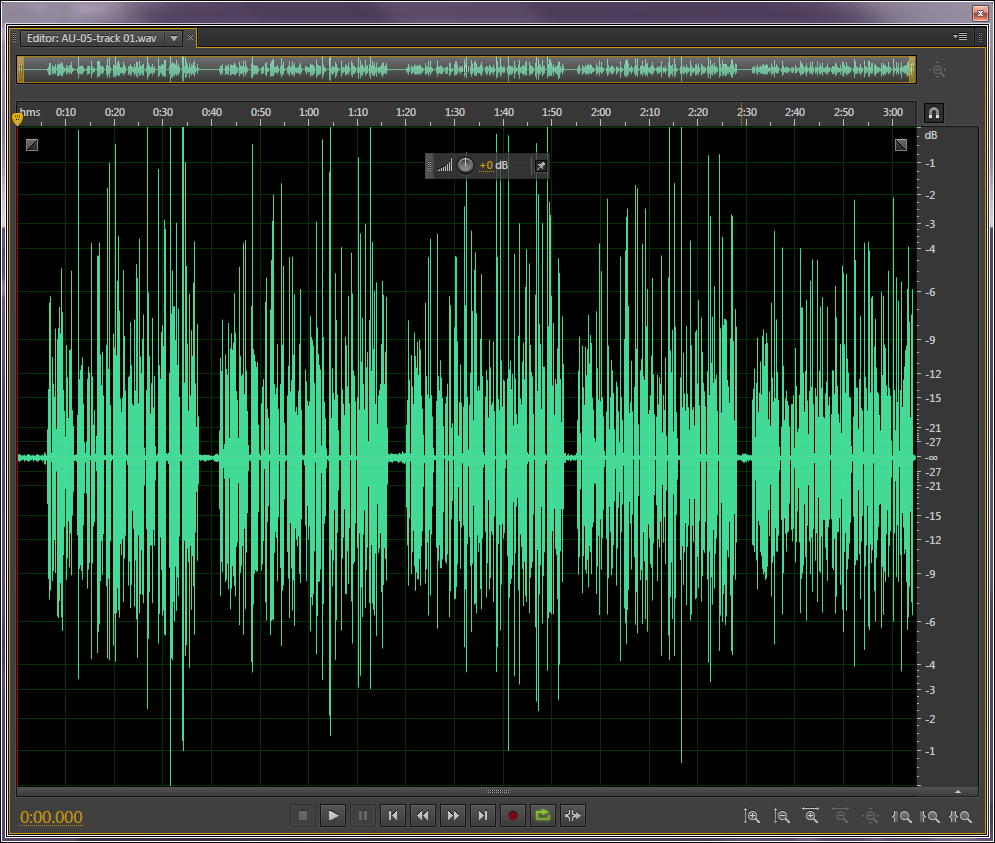
\includegraphics[width=0.5\textwidth]{pic-fivedoubles-01}}
\end{frame}   

\begin{frame}
Результат амплитудного анализа будет использоваться при решении вопроса о целесообразности борьбы с некоторыми шумами, искажениями, и при выборе параметров динамической обработки записанного сигнала.

~

Сбор статистической информации о волновой форме осуществляется с помощью окна \textit{Amplitude Statistics}, открываемого командой \textit{Window > Amplitude Statistics}.

~

Окно содержит три вкладки: 
\begin{itemize}
\item \textit{General}~--- статистическая информация о параметрах волновой формы;
\item \textit{RMS Histogram}~--- гистограмма (распределение значений) отсчетов волновой формы;
\item \textit{RMS Settings}~--- настройки для расчета гистограммы.
\end{itemize}
\end{frame}   

\begin{frame}
\centering{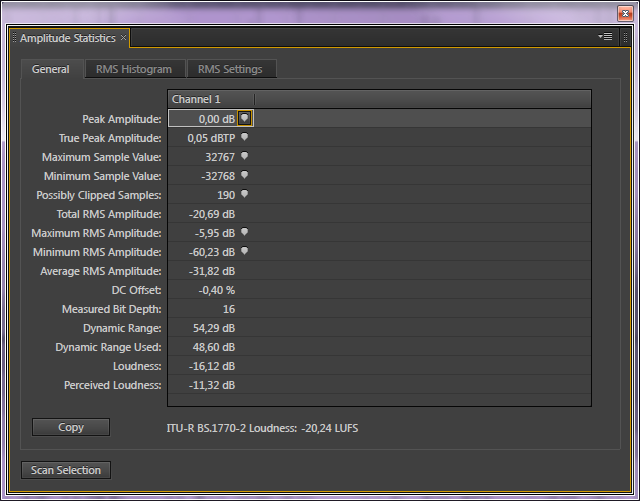
\includegraphics[width=0.75\textwidth]{pic-analis-01}}
\end{frame}   

\begin{frame}
\centering{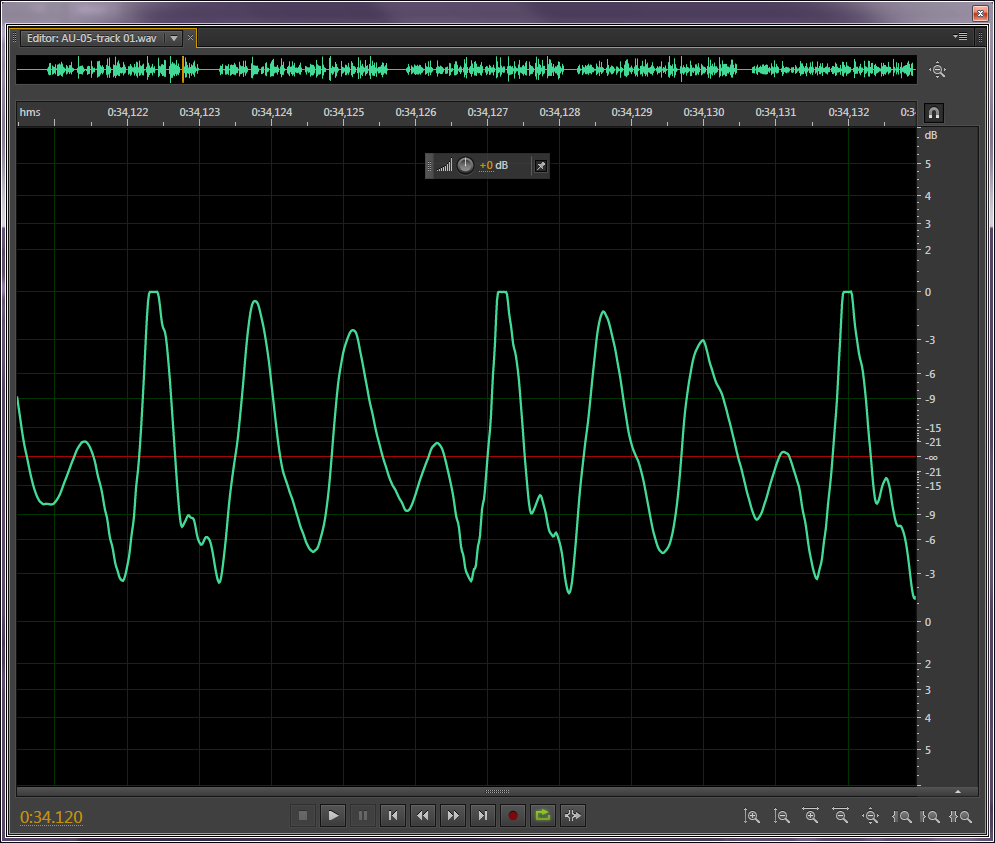
\includegraphics[width=0.75\textwidth]{pic-clipping-01}}
\end{frame}   

\begin{frame}
\centering{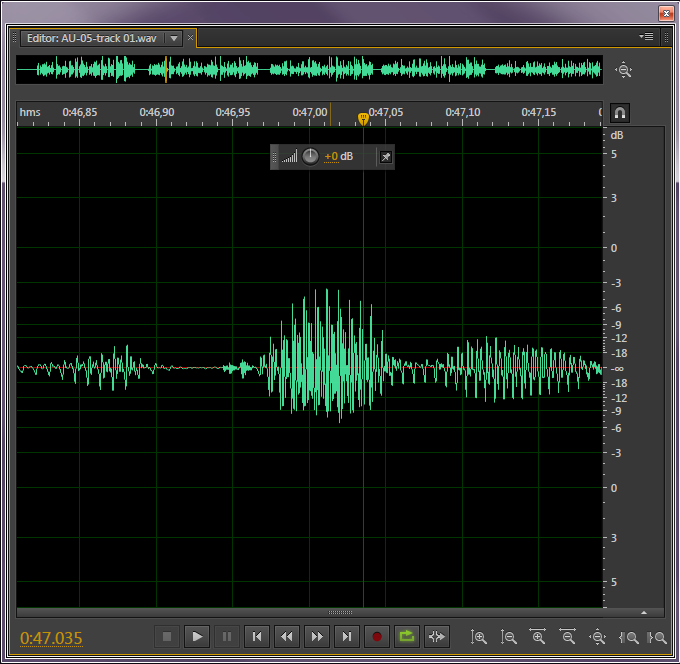
\includegraphics[width=0.7\textwidth]{pic-dcoffset-01}}
\end{frame} 

\begin{frame}
\centering{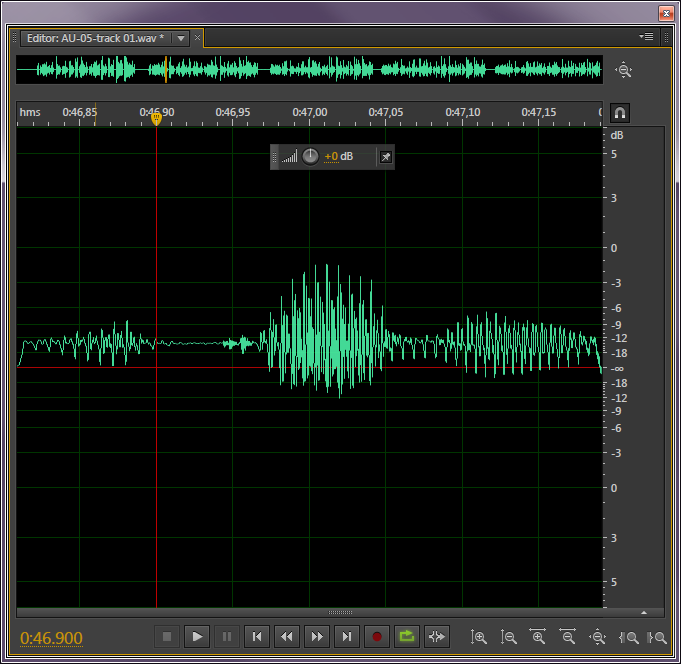
\includegraphics[width=0.7\textwidth]{pic-dcoffset-02}}
\end{frame}   

\begin{frame}
\begin{table}[ht]
  \caption{Результат сравнения пяти дублей}
  \begin{center}
  \begin{tabular}{|l|c|c|c|c|c|}
    \hline Параметр 				& Дубль 1 	& Дубль 2 	& Дубль 3 	& Дубль 4 	& Дубль 5\\
    \hline Clipped Samples & 108 		& 39 		& 4 		& 39 		& 0\\
    \hline Min RMS Amp 	& -57.77	& -56.76    & -60.22	& -60.05	& -56.58\\    
    \hline Loudness 				& -13.69	& -15.18	& -15.09	& -12.83	& -17.13\\    
    \hline 
  \end{tabular}
  \end{center}  
  \label{table-fivedoubles-01}
\end{table}
\end{frame}   

\begin{frame}
Гистограмма для звукового сиганла~--- изображение зависимости количества отсчетов, мощность которых попадает в заданный интервал, от величины громкости в децибелах.

\centering{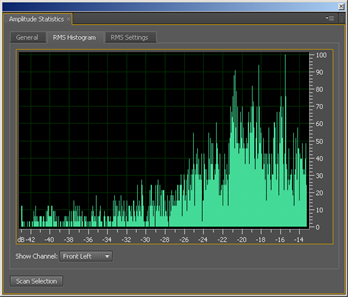
\includegraphics[width=0.6\textwidth]{pic-histogram-01}}
\end{frame}   

\begin{frame}
На основе анализа формы гистограммы можно получить следующую информацию:
\begin{itemize}
\item допустимый уровень порога при компрессии (-20 дБ);
\item уровень фоновых шумов (-45 дБ);
\item уровень ограничения для динамической обработки (-10 дБ).
\end{itemize}
\centering{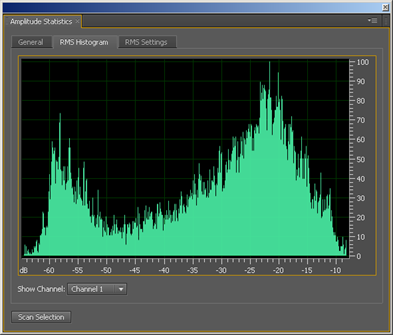
\includegraphics[width=0.6\textwidth]{pic-histogram-02}}
\end{frame}  

\begin{frame}
Команда \textit{View > Show Spectral Frequency Display} включает режим отображения спектрограммы сигнала в виде градаций яркости и цвета. По горизонтальной оси отложено время, по вертикальной~--– частота. Цвет и яркость точки зависят от уровня спектральной составляющей в анализируемом сигнале на той или иной частоте (чем ярче~--- тем выше уровень). 
\centering{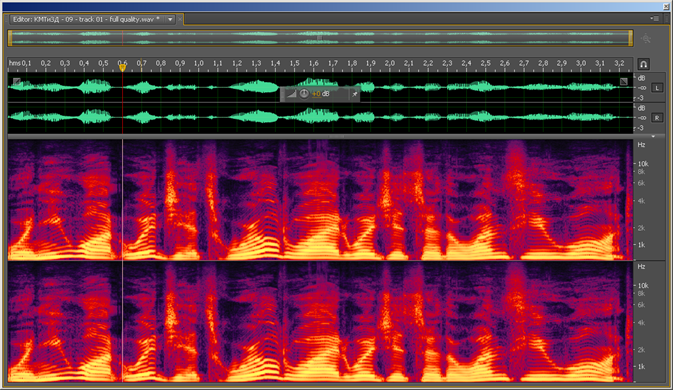
\includegraphics[width=0.7\textwidth]{pic-spectrogram-01}}
\end{frame} 

\begin{frame}
Просмотр сигнала в режиме \textit{Spectral Frequency Display} позволяет визуально определить шумы или отдельные искажения, такие как: 
\begin{itemize}
\item низкочастотный гул (А);
\item щелчок (B);
\item высокочастотное шипение (C).
\end{itemize}
\centering{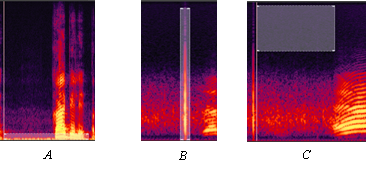
\includegraphics[width=0.9\textwidth]{pic-spectrogram-02}}
\end{frame} 

\begin{frame}
Тональные шумы могут возникать по разным причинам:
\begin{itemize}
\item собственный шум оборудования (обычно высокие частоты);
\item внешний фоновый шум~--- свист и жужжание;
\item наводки от сети переменного тока (частоты близки к частоте 50 Гц и ее нечетным гармоникам).
\end{itemize}

\centering{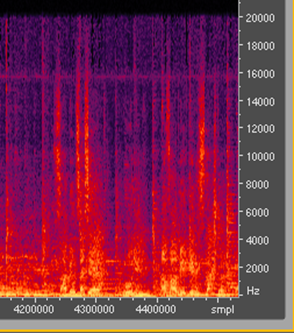
\includegraphics[width=0.3\textwidth]{pic-spectrogram-03}}
\end{frame}

\begin{frame}
В некоторых случаях наводки от сети электрического тока и прочие шумы оборудования проникают в область высоких часотот из-за наличия высших гармоник, что воспринимается на слух как жужжание. 

\centering{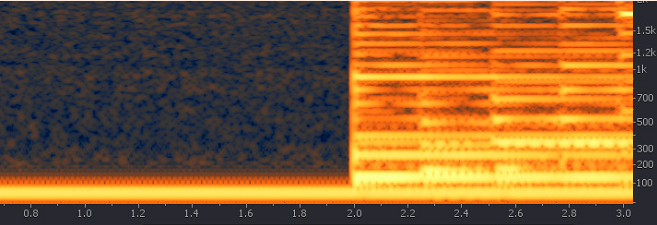
\includegraphics[width=0.75\textwidth]{pic-hum-01}}

~

\centering{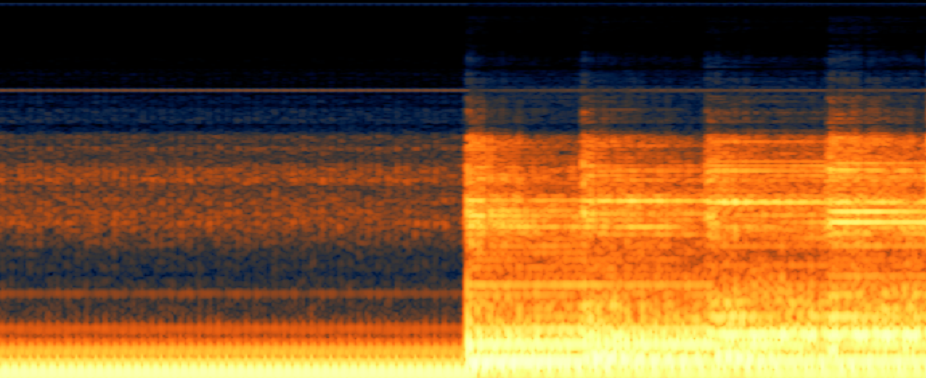
\includegraphics[width=0.75\textwidth]{pic-hum-02}}
\end{frame}

\begin{frame}
В отличие от гула и жужжания, шум шипения не сосредоточен на отдельных дискретных частотах. 

~

Шипение может иметь широкий спектр вплоть до всего частотного диапазона. Такой вид шума могут создавать проигрыватели магнитных лент и кассет, шум вентилятора или системы кондиционирования. 

\centering{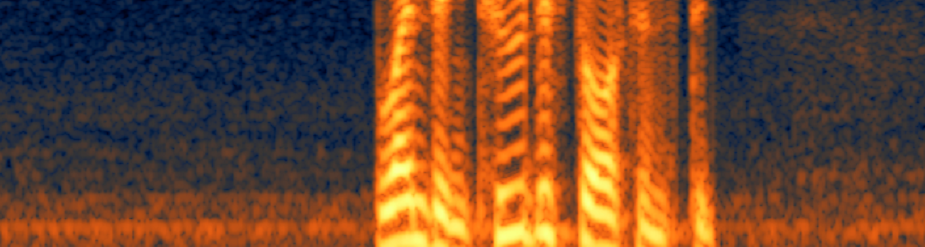
\includegraphics[width=0.75\textwidth]{pic-hiss-01}}
\end{frame}

\begin{frame}
В записи могут присутствовать нерегулярные и непериодические шумы, имеющие различную природу и частотный состав: одни в чем-то похожи на шипение, другие~--- на гул: кашель, чихание, шаги, гудок машины, звонок телефона и т.д. 

\centering{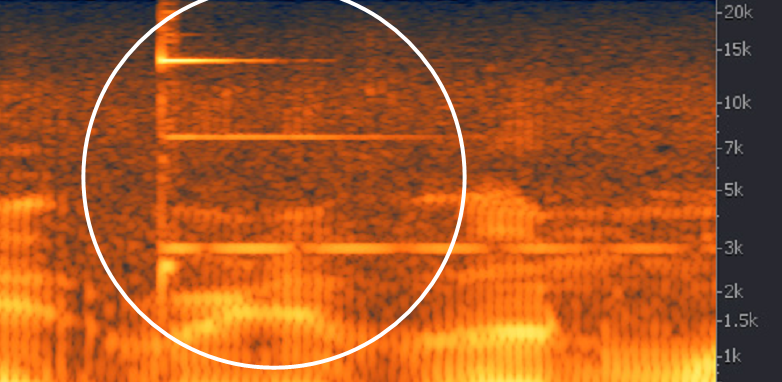
\includegraphics[width=0.5\textwidth]{pic-ringing-01}}

~

\centering{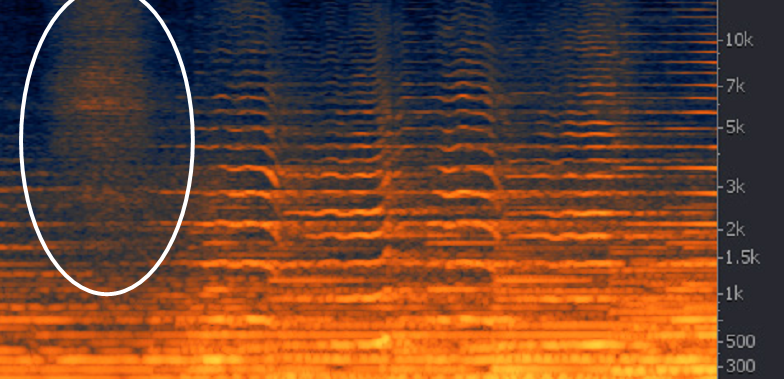
\includegraphics[width=0.5\textwidth]{pic-cough-01}}
\end{frame}

\begin{frame}
Командой \textit{Window > Frequency Analysis} открывается окно спектрального анализатора. При открытии окна происходит предварительный расчет спектра короткого фрагмента волновой формы или усредненный спектр выделенной области.

~

\centering{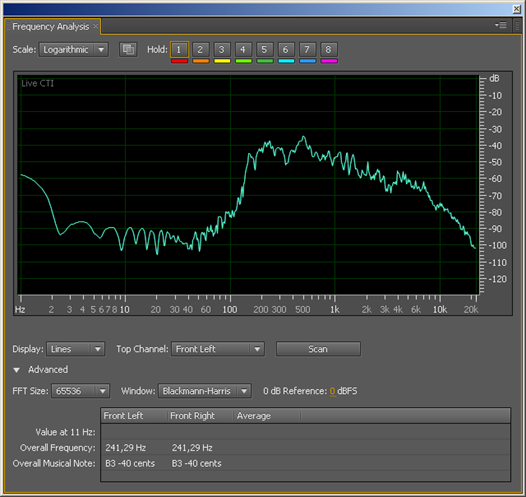
\includegraphics[width=0.45\textwidth]{pic-specter-01}}
\end{frame}

\begin{frame}
\centering{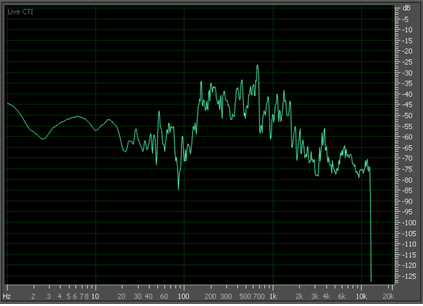
\includegraphics[width=0.5\textwidth]{pic-specter-03}}

При анализе спектра следует обращать внимание на следующее:
\begin{itemize}
\item верхняя частота ограничения спектра (на рис. около 13 кГц);
\item наличие наводок от сети переменного тока (частота 50Гц и ее нечетные гармоники);
\item наличие низкочастотного гула (подъем в области спектра ниже 100Гц, присутствует на рис.).
\end{itemize}
\end{frame}

\begin{frame}
\textit{Моносовместимость}~--- это свойство звукового файла, которое позволяет его прослушивать на монофоническом оборудовании. 

~

\centering{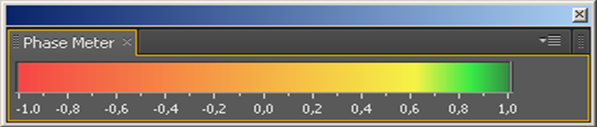
\includegraphics[width=0.5\textwidth]{pic-phase-01}}

~

Моносовместимость важна при передаче музыкальных композиций по радио и при сведении мультитрековой композиции. Определить на слух моносовместимость фонограммы без переключения в режим моно невозможно. 
\end{frame}

\subsection{Анализ звука VST-инструментами}

\begin{frame}
\textit{Virtual Studio Technology} (VST)~--- формат ресурсозависимых плагинов реального времени, которые подключаются к звуковым и музыкальным редакторам, секвенсорам и т. д.

Подключение VST-инструментов:
\begin{enumerate}
\item Установить VST-инструмент (как правило, программой-установщиком).
\item Подключить VST-инструмент в \textit{Adobe Audition}.
\end{enumerate}

\centering{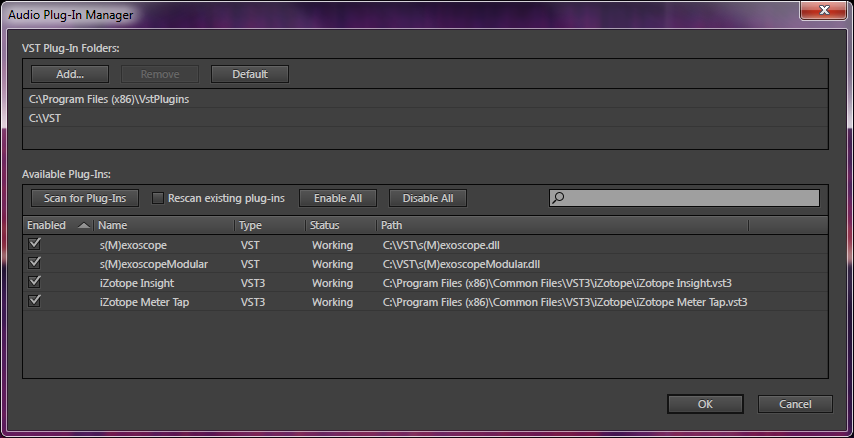
\includegraphics[width=0.75\textwidth]{pic-plugin-01}}
\end{frame}

\begin{frame}
Инструмент \textit{s(M)exoscope} является эффектом, реализующим цифровой осциллограф, который позволяет в режиме реального времени анализировать сигналлограмму и ее изменение под действием различных эффектов. 

~

\centering{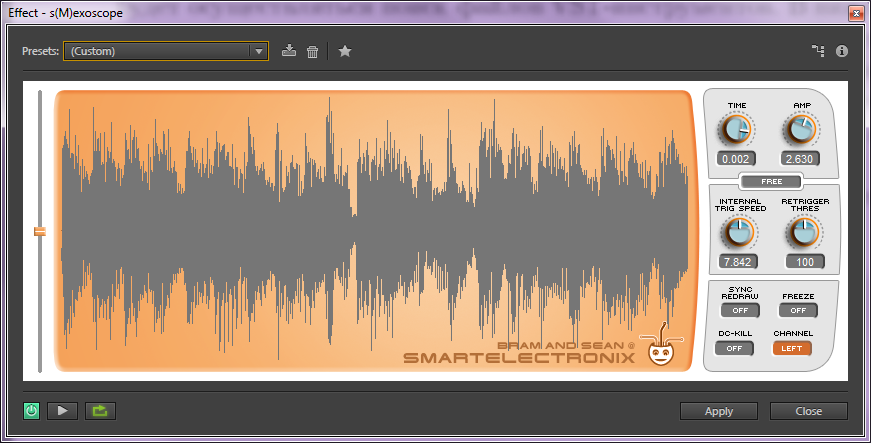
\includegraphics[width=0.75\textwidth]{pic-exoscope-01}}
\end{frame}

\begin{frame}
VST-инструмент \textit{Insight} компании \textit{iZotope} предназначен для проведения полноценного анализа звукового сигнала. 

\centering{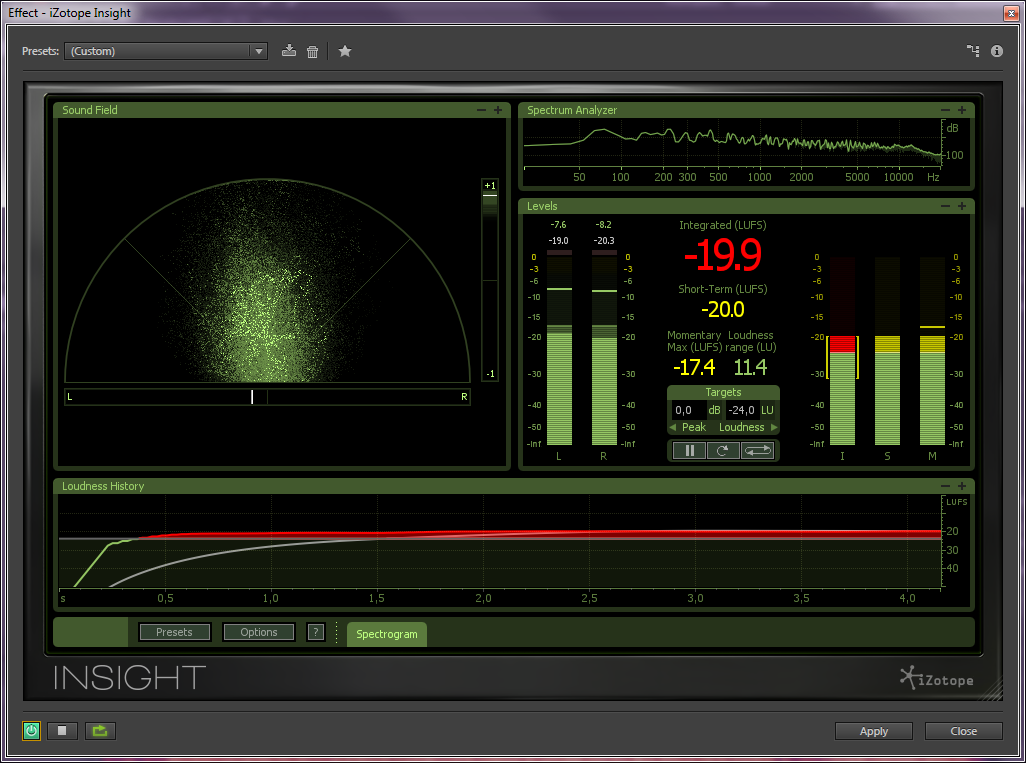
\includegraphics[width=0.75\textwidth]{pic-insight-01}}
\end{frame}

\begin{frame}
\textit{iZotope Insight} содержит следующие инструменты: 
\begin{itemize}
\item измеритель уровня сигнала;
\item измеритель громкости сигнала;
\item спектрограмма;
\item график амплитудно-частотного спектра;
\item анализатор фазы для двух- и многоканального звука;
\item график изменения громкости. 
\end{itemize} 

Измерители уровня (\textit{Level Meters} позволяют осуществлять мониторинг уровня сигнала в отдельных каналах. 

\centering{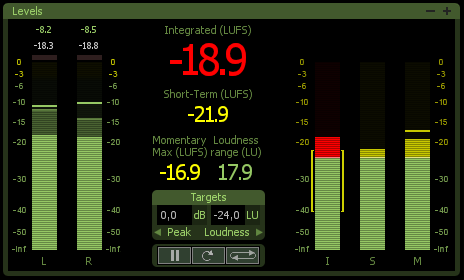
\includegraphics[width=0.5\textwidth]{pic-insight-04}}
\end{frame}

\begin{frame}
Инструмент \textit{Level Meters} отображает уровень сигнала, причем отображается одновременно и мгновенное значение (\textit{true-peak}) и уровень среднеквадратичной мощности (\textit{RMS, Root Mean Square}). Данный инструмент позволяет следить за изменением уровня сигнала с течением времени, а также обнаруживать клипирование сигнала.

\textit{Level Meters} позволяет измерять уровень сигнала следующими методами:
\begin{itemize}
\item \textit{Peak+RMS}~--- верхняя часть столбца соответствует измерению пиковой громкости сигнала, а нижняя и чуть более темная~--- среднеквадратичному уровню.
\item \textit{K-System}~--- метод измерения громкости звука с учетом прихоаккустических особенностей слуха человека. Существует несколько стандартных шкал: K-20, K-14, K-12, где за уровень 0 дБ приняты величины, соответственно, $-20$~дБ, $-14$~дБ и $-12$~дБ соответственно.
\end{itemize}

\end{frame}

\begin{frame}
\centering{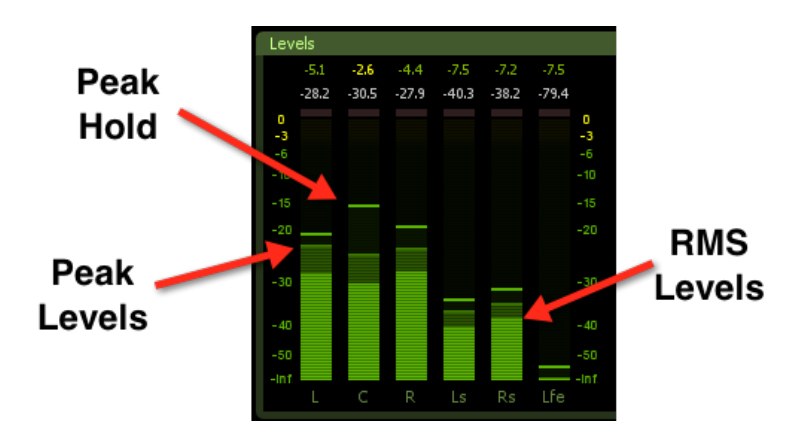
\includegraphics[width=0.65\textwidth]{pic-insight-05}}
  \begin{itemize}
  	\item K-12: для материала и небольшим динамическим диапазоном и подвергнутого сильной компрессии (например, для трансляции по радиоканалам);
  	\item K-14: для материала со средней степенью компрессии: поп и рок-музыка, аудио для цифрового видео и т.п.
  	\item K-20: для материала с большим динамическим диапазоном: запись концертного исполнения музыки, "<аудиофильские"> записи, симфоническая музыка и аудио в формате шестиканального звука.
  \end{itemize}
\end{frame}

\begin{frame}
(\textit{Loudness Meters}) осуществляют измерение громкости в соответствии с рекомендациями интернациональных стандартов. 

Существуют следующие методы расчета громкости (рис. \ref{pic-insight-07}):
\begin{itemize}
\item мгновенная громкость (\textit{Momentary}): расчет громкости на интервале в 400~мс. Данное значение отображается в столбце с литерой "<M">. 
\item максимум мгновенной громкости (\textit{Momentary Max}): максимальное значение из всех рассчитанных значений мгновенной громкости за прошедший период времени; данное значение отображается в поле \textit{Momentary Max}. 
\item краткосрочная громкость (\textit{Short-term}): расчет громкости на интервале в 3~сек.  Данный параметр удобен для анализа тренда громкости сигнала и отображается в стоблце с литерой "<S">.
\item суммарная громкость (\textit{Integrated}): расчет громкости производится на бесконечном отрезке времени (т.е. фактически усредняется на всем времени сигнала). Данный параметр отображается в стоблце с литерой "<I"> и в одноименном поле.
\end{itemize}
\end{frame}

\begin{frame}
\begin{itemize}
\item динамический диапазон громкости (\textit{Loudness Range}): отношение максимальной к минимальной громкости сиганала на всем периоде его звучания, выражается в единицах громкости (\textit{Loudness Units}, \textit{LU}). 1~\textit{LU} равен 1~дБ.
\end{itemize}
\centering{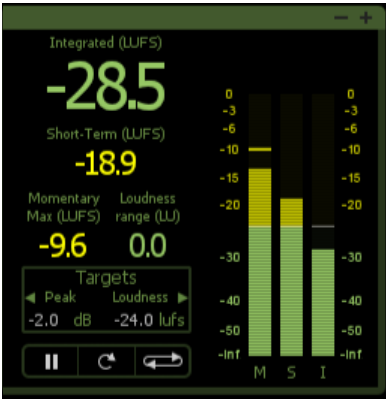
\includegraphics[width=0.4\textwidth]{pic-insight-07}}
\end{frame}

\begin{frame}
График изменения громкости \textit{Loudness History Graph} позволяет выполнять мониторинг тренда изменения громкости на протяжении всего времени сигнала. 

~

На графике могут отображаться: краткосрочная громкость, моментальнная громкость и суммарная громкость, а также случаи превышения суммарной громкостью заданного порога (\textit{Loundness Target}).

~

\centering{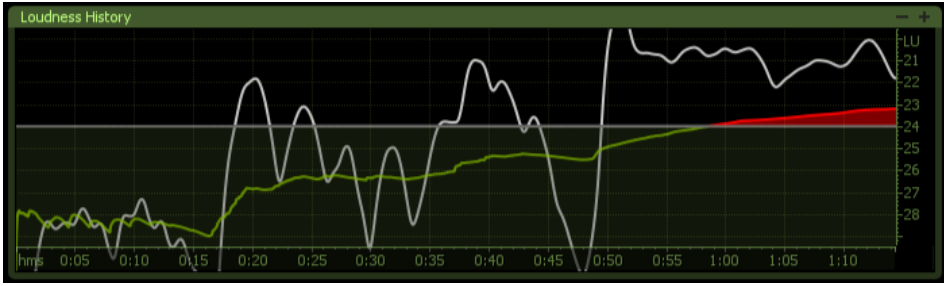
\includegraphics[width=0.75\textwidth]{pic-insight-08}}
\end{frame}

\begin{frame}
{Вектороскоп} позволяет анализировать анализировать различие между двумя каналами стерео сигнала при помощи графика в полярных координатах: полярный угол определяется разностью фаз каналов, а полярный радиус~--- суммой амплитуд каналов.  

~

\centering{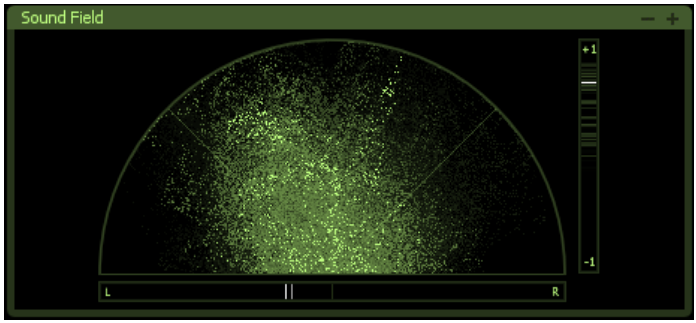
\includegraphics[width=0.75\textwidth]{pic-insight-09}}
\end{frame}

\begin{frame}
Вектороскоп имеет несколько режимов отображения сигнала:
\begin{itemize}
\item отсчеты в полярных координатах (\textit{Polar Sample Vectorscope});
\item уровень каналов в полярных координатах (\textit{Polar Level Vectorscope});
\item в виде фигур Лиссажу (\textit{Lissajous Vectorscope});
\end{itemize}

\centering{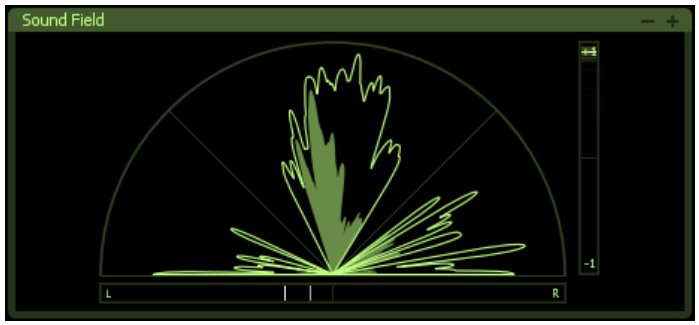
\includegraphics[width=0.75\textwidth]{pic-insight-10}}
\end{frame}

\begin{frame}
\centering{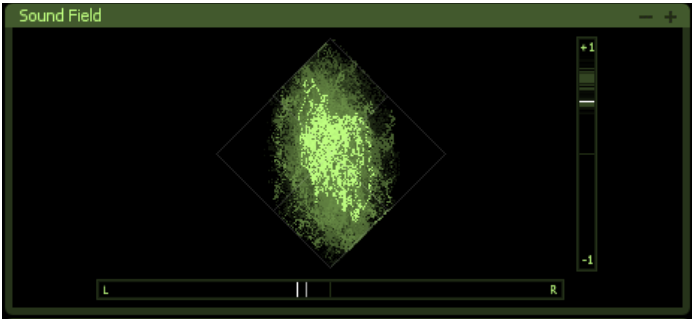
\includegraphics[width=0.75\textwidth]{pic-insight-11}}
\end{frame}

\begin{frame}{Спектрограмма} 
В эффекте \textit{iZotope Insight} спектрограмма может отображаться как в двумерном, так и в трехмерном виде и поддерживает операции вращения и масштабирования. 

\centering{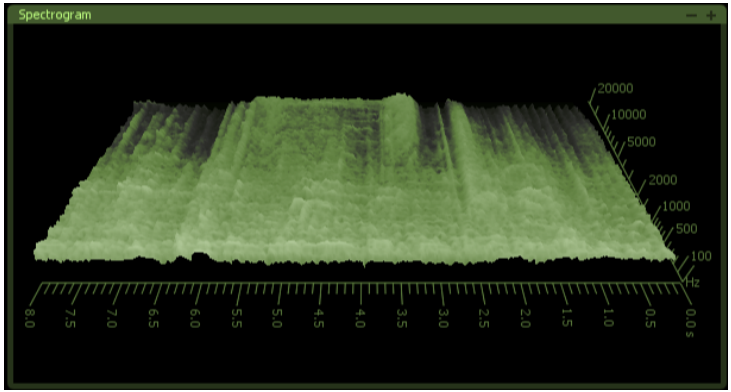
\includegraphics[width=0.8\textwidth]{pic-insight-12}}
\end{frame}

\begin{frame}
\centering{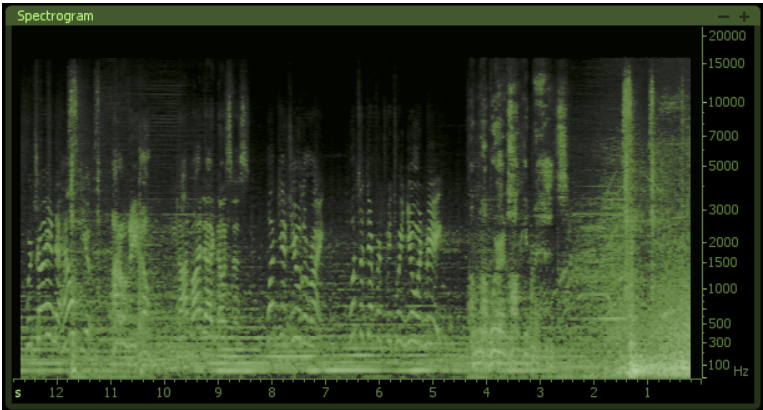
\includegraphics[width=0.8\textwidth]{pic-insight-13}}
\end{frame}

\begin{frame}{Спектральный анализатор} 
Классический график амплитудно-частотного спектра позволяет выполнять частотный анализ в режиме реального времени. 

~

\centering{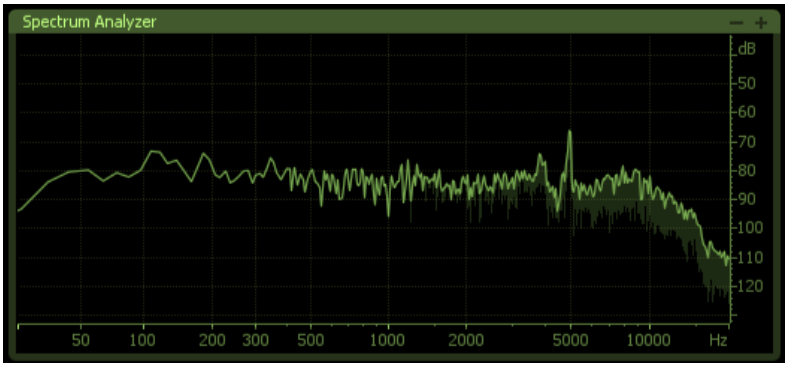
\includegraphics[width=0.75\textwidth]{pic-insight-14}}
\end{frame}

\begin{frame}
График поддерживает масштабирование по обоим осям и может отображаться в следующих режимах:
\begin{itemize}
\item \textit{Linear}: в виде непрерывной линии;
\item \textit{1/3 Octave}: в виде гистограммы с шириной полосы в $1/3$ октавы; 
\item \textit{Full Octave}: в виде гистограммы с шириной полосы в $1$ октаву;
\item \textit{Critical bands}: в виде гистограммы с переменной шириной полосы, соответствующей ширине критической полосы, равной $1$ Барк. 
\end{itemize}

\centering{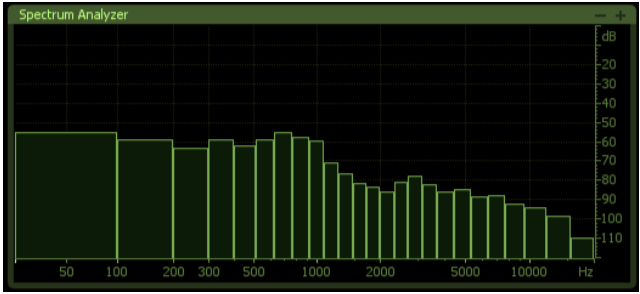
\includegraphics[width=0.75\textwidth]{pic-insight-15}}
\end{frame}

\end{document}
